\documentclass[aps,prab,reprint,superscriptaddress,showpacs,showkeys,letter]{revtex4-1}
%\documentclass[aps,prab,preprint,superscriptaddress,showpacs,showkeys]{revtex4-1}
\usepackage{graphicx}% Include figure files

\usepackage{dcolumn}% Align table columns on decimal point
\usepackage{bm}% bold math
\usepackage{amsmath}
%\usepackage{subfigure}
\usepackage[caption=false]{subfig}
\usepackage[none]{hyphenat}
\usepackage{color}
\usepackage{mathrsfs}
\usepackage{epstopdf}
\usepackage{amssymb}
\usepackage{mathrsfs}
\usepackage{url}
%\usepackage{hyperref}
\usepackage[colorlinks,linkcolor=blue]{hyperref}
\captionsetup[subfigure]{labelformat=brace}

\begin{document}

\title{Manual of FASTION code}
\author{Chao Li }
\email{supperli.imp@gmail.com}
\date{December 2019}



\maketitle

\section{Introduction}
The code FASTION was developed to study the beam-ion interaction in electron rings. In electron accelertors, ions could be repeated generated due to collision ionization when  electron bunches passed by. The ions generated would interact with the tail bunch leading to a "head-tail" coupled beam motion. Beside the beam-ion interaction, several potential APIs are also designed to keep possible potential to include more physical mechanisms into account, as impedance and wakefield.   
This manual will  give basic models and equations used in the code, and setting to used the code are also explained.     

\section{Beam-ion interaction}
Denoting $P$ and $T$ as the vacuum pressure and temperature, the molecules density $n$ in the accelerator can be obtained from the general gas equation, 
\begin{eqnarray}
\label{eq2.1}
P N_A= nRT,
\end{eqnarray}
where $R$ and $N_A$ are the ideal gas constant and the Avogadro number. Denote $\sum$ as the ionization cross-section, $N_b$ as the number of electron particles passing by, the number of ionization ions per unit length is 
\begin{eqnarray}
\label{e2.2}
\lambda = \sum n N_b.
\end{eqnarray}

For simplicity, the interaction between ions and beam is assumed taking place at lumped interaction locations, and the ions are assumed not to move longitudinally. 
When beam passes through interaction points bunch by bunch, the ions generated  are randomly distributed  in the same range as the size of the electron bunch passing by. At the interaction point, the accumulated ions are kicked by the passing bunched electron particles and then drift freely until next electron bunch comes.  The motion equations of the $i$th accumulated ion $\vec X_i$ and the $k$th electron particle in the $j$th bunch $\vec x_{k;j}$ can be expressed as
\begin{eqnarray}
\label{eq2.3}
\frac{d^2\vec X_i}{dt^2} +K_i(s) \vec x_{k;j} + \sum_{k=0}^{N_j} \vec F_C(\vec X_i - \vec x_{k;j}) =0 \nonumber  \\
\frac{d^2\vec x_{k;j}}{ds^2} + K_e(s) \vec x_{k;j} +\sum_{i=0}^{N_i} \vec F_C(\vec x_{k;j} - \vec X_i ) =0,
\end{eqnarray}
where $\vec F_C$ is the Coulomb force between the ions and electron particles, $K_i(s)$ and $ K_e(s)$ represent the lattice focusing strength on ion and beam particle.

\begin{figure}[t]
\centering
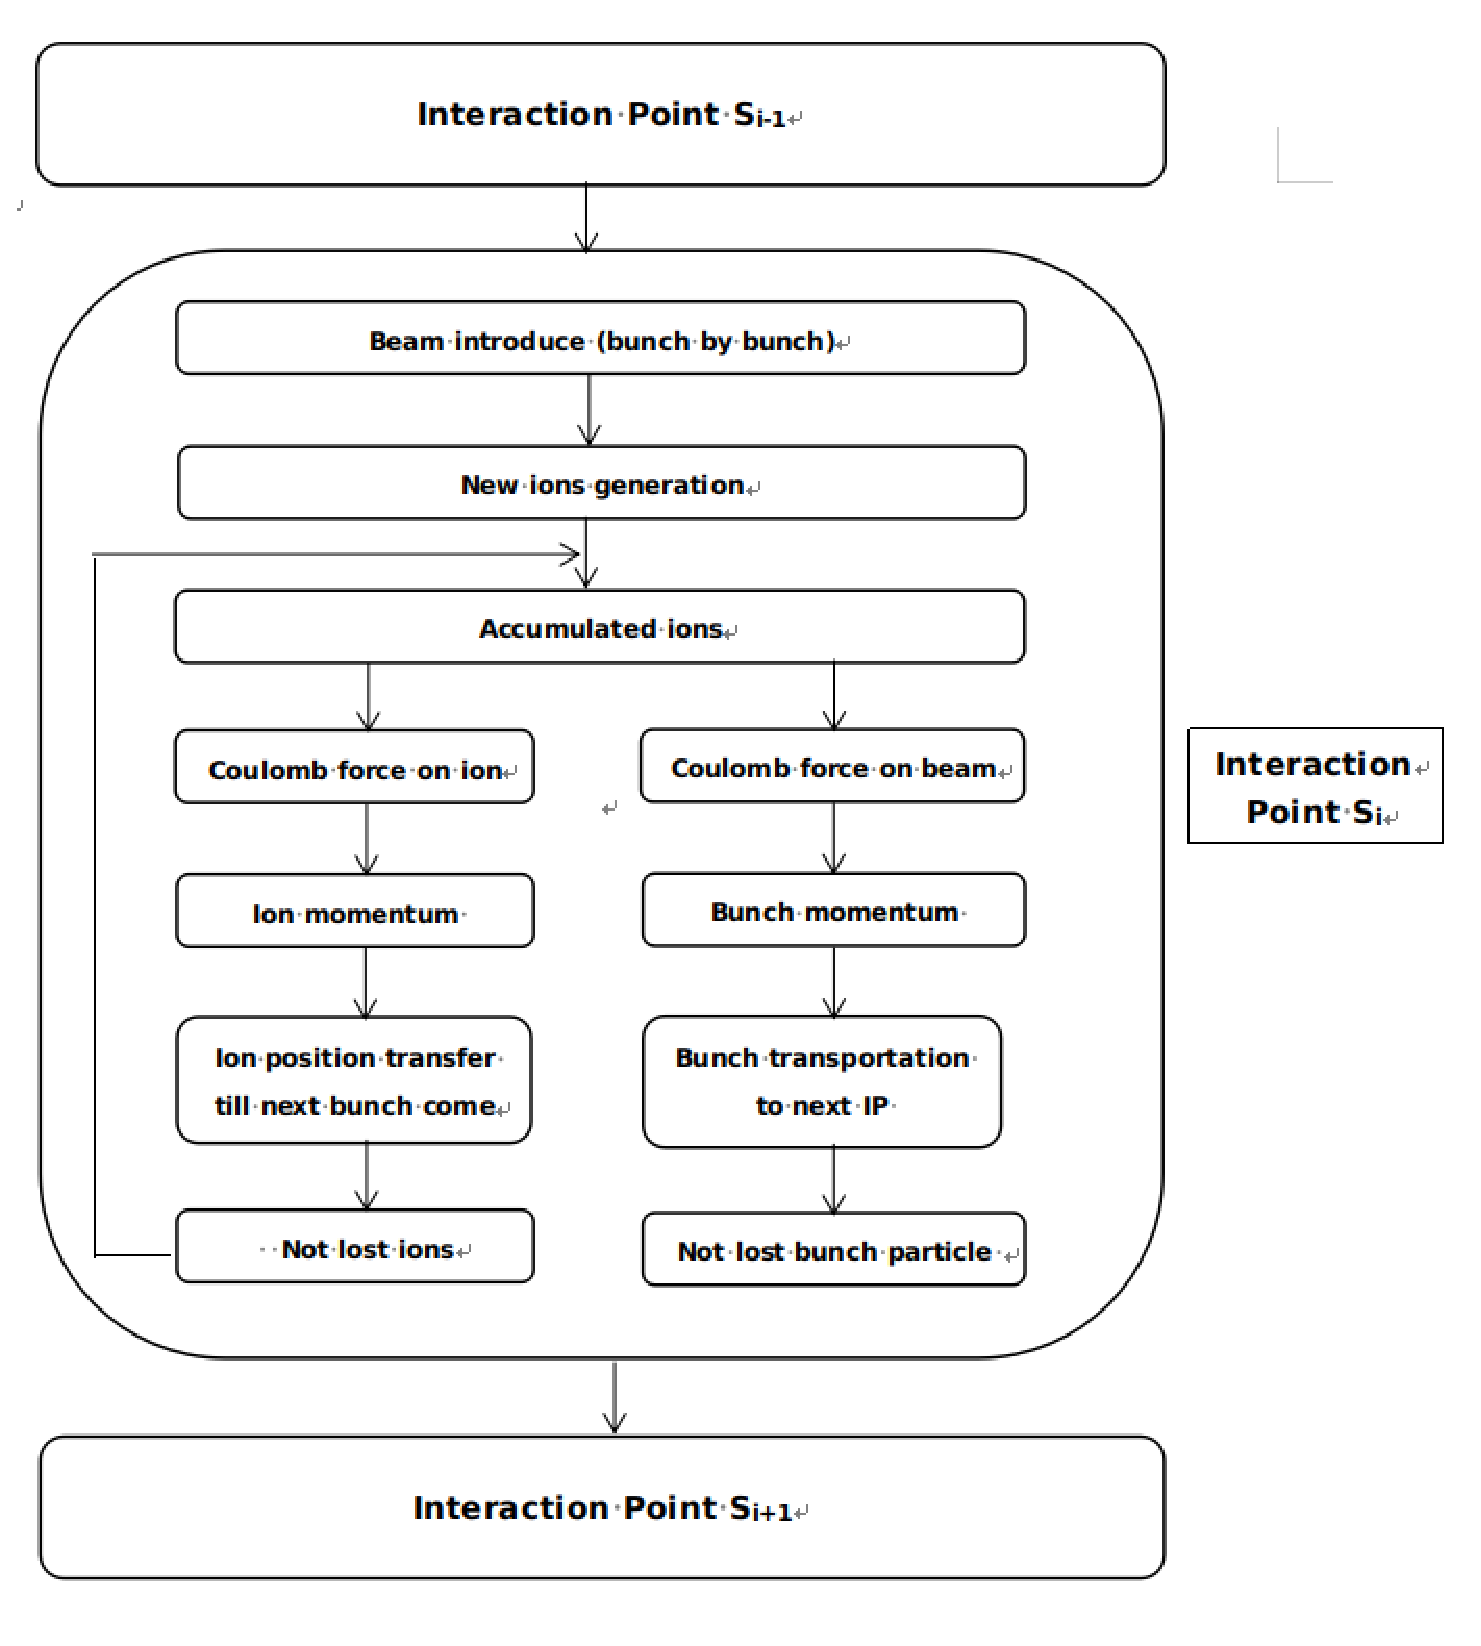
\includegraphics[width=1\linewidth]{Fig1.eps}
\caption{Logic flow of the beam-ion interaction in simulation at the interaction points. }
\label{fig:fig1}
\end{figure}

In the FASTION code, the 2D Bassetti-Erskine formula is use to get the space charge potential of the  electron bunch, since the Gaussian profile assumption is rather good for electron bunch. At the interaction point $s_i$, 
\begin{eqnarray}
\label{eq2.5}
E_{C,y}( \vec  x ) + I E_{C, x}(\vec x) &=& \frac{n_b}{2\epsilon_0\sqrt{2\pi (\sigma_x^2-\sigma_y^2)}} 
\{w(\frac{x+Iy}{\sqrt{2(\sigma_x^2-\sigma_y^2)}}) \nonumber  \\
&-&\exp(-\frac{x^2}{2\sigma_x^2}-\frac{y^2}{2\sigma_y^2}) \nonumber  \\
 &+& w(\frac{x\frac{\sigma_y}{\sigma_x}+Iy\frac{\sigma_x}{\sigma_y}}{\sqrt{2 (\sigma_x^2-\sigma_y^2)}}) \} \delta(s_i), 
\end{eqnarray}
where $n_b$ is the line density of the electron beam, $w(z)$ is the complex error function, $\sigma_x$ and $\sigma_y$ are the beam rms size in horizontal and vertical direction, $x$ and $y$ are the distance from ions to the bunch centroid, $I$ is the complex unit. Substituting Eq.~\ref{eq2.5} into Eq.~\ref{eq2.3}, the explicit momentum change of ions at the interaction point is 
\begin{eqnarray}
\label{eq2.6}
\Delta p_{i,y} + I \Delta p_{i,x} &=& \frac{2 n_br_em_ec}{\gamma_e} (E_{C,y} + I E_{C, x}), 
\end{eqnarray}
where $r_e$ is the classical electron radius, $m_e$ is the electron mass, $c$ is the speed of light, $\gamma_e$ is the relativistic factor of electron beam. Since the ions are much heavier than the electron, the lattice focusing $K_i(s)$ can be ignored. 

As to the space charge potential well generated by the ions, since the ions distribution is usually not a Gaussian type and the ion particles almost occupy the whole pipe, in principle the Bassetti-Erskine formula is not suitable anymore. A self-consistent particle-in-cell (PIC)  solver or ion density profile fitting is required. In the FASTION code, a  compromise approach is applied. The ions distribution is truncated at 10 rms bunch size. The rms and centroid information of the truncated ion distribution are substituted in the Bassetti-Erskine formula to get the Coulomb potential.  When one electron bunch particles passes by, the transverse momentum and position of the accumulated ions are updated according to the time interval until the next bunch comes. As to the bunched electron particles, after the momentum kicks induced by the accumulated ions, they are transferred to the next interaction point by applying the linear transport matrix. 

\section{Bunch-by-bunch feedback}
The bunch-by-bunch feedback based on the FIR filter is an effective way to cure the coupled bunched instability. It detects transverse or longitudinal centroid positions of beam bunches, processes the positions data to create  kicker signals, and adds transverse or longitudinal kicks to the beam particles to damp its oscillations. 
Eq.~\ref{eq3.1} is the general form of a FIR filter
\begin{eqnarray}\label{eq3.1}
\Theta_n= \sum_{k=0}^{N}a_k x_{n-k},
\end{eqnarray}
where $a_k$ represents the filter coefficient, $x_{n-k}$ and $\Theta_n$ are the input and output of the filter, corresponding to beam position data at the $(n-k)$th turn and kick strength on the beam at the $n$th turn. The number of the input data $N+1$ is defined as taps. Following the approaches shown in Ref.~\cite{21}, the time domain least square fitting (TDLSF) method is used to get the filters  coefficients $a_k$. 

In the FASTION code, the beam momentum change by the bunch-by-bunch feedback at the $n$th turn is modeled as 
\begin{eqnarray}\label{eq3.5}
\Theta_{x,n}= K_x \sum_{k=0}^{N}a_{k,x} x_{n-k}, \nonumber  \\
\Theta_{y,n}= K_y \sum_{k=0}^{N}a_{k,y} y_{n-k},
\end{eqnarray}
The  beam motion transfer function in one turn including feedback is 
\begin{eqnarray}\label{eq3.6}
 { 
 \left[
 \left( 
 \begin{array}{c} 
 x_{n+1}  \\ 
 x'_{n+1}  \\
  y_{n+1}  \\ 
 y'_{n+1}  
 \end{array} 
 \right)
 \right ]}
 =M_0{ 
 \left[
 \left(  
 \begin{array}{cc} 
 x_{n}  \\ 
 x'_{n}  \\
  y_{n}  \\ 
 y'_{n}  
 \end{array}
  \right)
 +  
 \left(  
 \begin{array}{cc} 
 0  \\ 
 \Theta_{x,n} \\
 0  \\ 
 \Theta_{y,n} \\ 
 \end{array}
   \right)
 \right ]},
\end{eqnarray}
 where $M_0$ is the one turn matrix at the  kicker.


\section{Synchrontron radiation damping and excitation}
Following approaches used in Hirata’s BBC code and Yuan Zhang's Beam-beam code , the transportation through the arc consists of the following maps
\begin{itemize}
\item[1. ] From accelerator coordinates to normalized coordinates; 
\item[2. ] Transportation with synchrotron radiation; 
\item[3. ] From normalized coordinates to accelerator coordinates.
\end{itemize}

Basically, in the first setp, it follows, 
\begin{eqnarray}\label{eq4.1}
X = BRHx
\end{eqnarray}
where H is the dispersion matrix, R is the Teng matrix, B is the Twiss matrix. At the second step, with synchrotron radiation, the arc transportation in the normalized coordinates is
\begin{eqnarray}\label{eq4.2}
\left( 
 \begin{array}{c} 
 X_1  \\ 
 X_2  
 \end{array} 
 \right)
 = 
 \lambda_u m_u\left(  
 \begin{array}{cc} 
 X_1  \\ 
 X_2  
 \end{array}
  \right)
 + 
 \sqrt{\epsilon_x(1-\lambda_u^2)}  
 \left(  
 \begin{array}{c} 
 \hat{r}_1 \\
 \hat{r}_2  
 \end{array}
   \right)}, \nonumber \\
  \left( 
 \begin{array}{c} 
 X_3  \\ 
 X_4  
 \end{array} 
 \right)
 = 
 \lambda_{\nu} m_{\nu}\left(  
 \begin{array}{cc} 
 X_3  \\ 
 X_4  
 \end{array}
  \right)
 + 
 \sqrt{\epsilon_y(1-\lambda_{\nu}^2)}  
 \left(  
 \begin{array}{c} 
 \hat{r}_3 \\
 \hat{r}_4  
 \end{array}
   \right)},  \nonumber \\
  \left( 
 \begin{array}{c} 
 X_5  \\ 
 X_6  
 \end{array} 
 \right)
 = 
 \left(  
 \begin{array}{cc} 
 1  & 0 \\ 
 0  & \lambda_{w}^2
 \end{array}
  \right) m_{w}
 \left(  
 \begin{array}{cc} 
 X_5  \\ 
 X_6  
 \end{array}
  \right)
 + 
 \sqrt{\epsilon_z(1-\lambda_{w}^4)}  
 \left(  
 \begin{array}{c} 
 0 \\
 \hat{r}_5  
 \end{array}
   \right)}  
\end{eqnarray}
Here $\hat{r}$ are are independent Gaussian random variables with
unit variance, $\lambda_i $=$\exp(-1/T_i)$  with $T_i$ the damping time in unit of the number of turns, and $\epsilon_z$ is calculated as $\sigma_z \sigma_e$. At the last step,
\begin{eqnarray}\label{eq4.3}
x = H^{-1}R^{-1}B^{-1} X
\end{eqnarray}

\section{Settings of the FASTION}
FASTION is developed with C++. It is an open source tool which can be download with links \url{https://github.com/ChaoLiIHEP/FASTION}. With the make file, the code can be  can be complied if all of the source scripts and head files are located in the same directory. Only the GSL \cite{22} library are required. 

\subsection{settings in input.dat}



\begin{itemize}
\item CircRing [m]: circumference of ring; 
\item WorkQx: workiing point in x direction; 
\item WorkQy: workiing point in y direction;
\item WorkQz: workiing point in z direction; It is a dummy parameter in beam-ion interaction simulation;
\item RFBaseFrequency [Hz]: fundamental frequency of the RF cavity;
\item CorssSectionEI [m$^2$]: ionization cross-section; Currently, the CO is used as the default gas in simulation; If the other ions are required, the mass number 28 also have to be modified in bunch.cpp, line 708 and line 573;
\item PipeAperatureX [m]: pipe aperture in x direction;
\item PipeAperatureY [m]: pipe aperture in y direction;
\item PipeAperatureR [m]: pipe aperture R; 
the spare boundaries with $PipeAperatureX$ and $PipeAperatureY$ are used as default beam and ions loss criteria;
\item ionlossboundary: default value in unit of beam rms size used as  ion loss   criteria;
\item ionMaxNumber: if accumulated ions number si larger than  $ionMaxNumber$, program will be quit automatically;
\item numberofIonBeamInterPoint: number of ionteraction points used in program. The program will read the data in $InterPointParameter.dat$ automatically, in which $numberofIonBeamInterPoint$ sets of local parameters have to be supplied; 
\item electronBeamEnergy: electron beam energy;
\item rmsBunchLength [m]: initial rms bunch length;
\item rmsEnergySpread [rad]: initial rms bunch energy spread; The bunch initial distribution is truncated within the ragne of  3 sigma.  
\item macroEleNumPerBunch: number of macro-particles used to represent the electron bunch; 
\item distributionType: flag for initial electron beam distribution in transverse direction; $distributionType=1$: kV; $distributionType=1$: Water Bag; $distributionType=3$: Gaussion truncated within 3 sigma;
\item initialDisDx [m]: Max initial displacement error of electron bunch in x direction; errors are randomly generated within the range  $initialDisDx$
\item initialDisDy [m]: Max initial displacement error of electron bunch in y direction; errors are randomly generated within the range  $initialDisDy$;
\item nTurns: tracking turns in simulations;
\item macroIonNumberGeneratedPerIP: number of macro-ions generated for each collision at interaction point.
\item trainNumber: train number at the ring; 
\item totBunchNumber: total bunch number in rings
\item bunchNumberPerTrain: it is an array; $trainNumber$ valeus have to be supplied; 
\item trainGaps:  it is an array; $trainNumber$ valeus have to be supplied;
\item SynRadDampingFlag: Flag to turn on the and off the synchrontron radiation damping and excitation; $SynRadDampingFlag=1$ the values $synchRadDampTimex$, $synchRadDampTimey$ and $synchRadDampTimez$ are used in simulation. 
\item synchRadDampTimex: damping time in x direction in the unit of turns. It is a dummy variabel if $SynRadDampingFlag=0$;
\item synchRadDampTimey: damping time in y direction in the unit of turns.  It is a dummy variabel if $SynRadDampingFlag=0$;
\item synchRadDampTimez: damping time in z direction in the unit of turns.  It is a dummy variabel if $SynRadDampingFlag=0$;
\item  current: total beam current;
\item  emittanceX [m rad]: beam rms emittance in x direction;
\item kappa: emittance couping factor; with $kappa$ the emittance in y direction is $emittanceX*kappa$
\item bunchBinNumberZ: number of bins for each bunch. It is used to calculate the beam-impedance interaction. Curretly, it is a dummy variable and not used. 
\item fIRBunchByBunchFeedbackFlag: flags to take the fir filter into account. $fIRBunchByBunchFeedbackFlag=0$ bunch-by-bunch is not taken into account; if $fIRBunchByBunchFeedbackFlag=1$, the code will read the parameter in $FIR_input.dat$ to get the paramters of filter, kickers and pickups
\item printInterval: interval in unit of turns to print the beam data;
\itme intevalofTurnsIonDataPrint: interval in unit of turns to print the ion data;
\item calSettings: index for simulations settings; if  $calSettings=1$, the beam-ion effect is calculated;  if  $calSettings=2$, single bunch - longitudinal impedance interaction is simulated.
\end{itemize}

\bibliography{reference}
\end{document}
